% ============================================================
% FILE RỜI — CHƯA \input VÀO main.tex
% Nội dung: đặc tả use case toàn hệ thống + nhúng ảnh sơ đồ use case.
% Vị trí chèn khi merge: chapters/chuong5-phantich-thietke.tex, thay thế
% dòng "% TODO: vẽ use case diagram..." trong \subsection{Mô hình hóa tương
% tác} (sec:sddchitiet).
%
% !!! CẢNH BÁO QUAN TRỌNG VỀ RBAC !!!
% Bản đặc tả và 5 file diagram HTML (tools/design/usecase-*.html) ĐÃ VẼ
% TRƯỚC ĐÓ dùng giả định "5 vai trò admin chuyên biệt" (admin_moderator,
% admin_compliance, admin_support, admin_ops, admin_inventory). Sau khi đọc
% lại chuong4-hethong-dexuat.tex, RBAC THẬT của hệ thống chỉ có:
%   seller, buyer_retail, buyer_wholesale, ops_sourcing (bộ phận thu mua),
%   admin_moderator, admin_ops, và admin (super-admin gộp 2 vai trò admin).
% Tức là CHỈ 2 vai trò admin chuyên biệt (không phải 5), và có thêm 1 vai
% trò "ops_sourcing" (bộ phận thu mua) mà bản đặc tả/diagram cũ chưa có.
% => Bảng actor và đặc tả dưới đây đã được SỬA LẠI cho khớp RBAC thật.
% => 5 file diagram HTML trong tools/design/ CẦN VẼ LẠI cho khớp trước khi
%    render và nhúng chính thức — mục "Việc cần xác nhận" ở cuối file nêu rõ.
% ============================================================

\subsection*{Đặc tả Use Case}
\label{subsec:usecase}

Mục này trình bày sơ đồ use case tổng quát và theo từng tác nhân, cùng bảng đặc tả cho các use case chính, bám theo mã FR tại mục~\ref{sec:yeucauchucnang} và các quy trình nghiệp vụ tại mục~\ref{sec:quytrinhnghiepvu}.

\subsubsection*{Danh sách tác nhân (actor)}

Bảng~\ref{tab:actor-usecase} liệt kê các tác nhân, khớp với vai trò RBAC đã xác lập tại mục~\ref{sec:doituongnguoidung}.

\begingroup
\small
\renewcommand{\arraystretch}{1.25}
\begin{longtable}{L{4.0cm} L{3.0cm} L{6.5cm}}
\caption{Danh sách tác nhân trong sơ đồ use case}
\label{tab:actor-usecase} \\
\toprule
\rowcolor{tblheadbg}
\textbf{Tác nhân} & \textbf{Vai trò RBAC} & \textbf{Ghi chú} \\
\midrule
\endfirsthead
\toprule
\rowcolor{tblheadbg}
\textbf{Tác nhân} & \textbf{Vai trò RBAC} & \textbf{Ghi chú} \\
\midrule
\endhead
\bottomrule
\endfoot
Nhà cung cấp (nông dân/HTX) & \texttt{seller} & Tham gia cả hai luồng bán sỉ và bán lẻ (cung cấp hàng cho thu mua) \\
\rowcolor{tblaltbg}
Khách lẻ & \texttt{buyer\_retail} & Chỉ tham gia luồng bán lẻ (1P) \\
Khách sỉ (doanh nghiệp thu mua) & \texttt{buyer\_wholesale} & Chỉ tham gia luồng bán sỉ (3P) \\
\rowcolor{tblaltbg}
Bộ phận thu mua & \texttt{ops\_sourcing} & Vận hành nội bộ, riêng cho luồng bán lẻ (1P) --- ra quyết định thu mua theo lô \\
Quản trị viên kiểm duyệt & \texttt{admin\_moderator} & Kiểm duyệt hồ sơ, sản phẩm, chứng nhận \\
\rowcolor{tblaltbg}
Quản trị viên vận hành & \texttt{admin\_ops} & Xử lý vi phạm, khiếu nại, báo cáo thống kê, giám sát tồn kho/vận chuyển \\
Quản trị viên cấp cao & \texttt{admin} & Gộp toàn bộ quyền của \texttt{admin\_moderator} và \texttt{admin\_ops} (mục~\ref{sec:doituongnguoidung}, mục e3) \\
\rowcolor{tblaltbg}
Hệ thống AI \textit{(actor phụ)} & --- & Hỗ trợ gợi ý sản phẩm (FR12.1), dự báo (FR12.2), luật ngưỡng giám sát bất thường \\
Cổng thanh toán trung gian \textit{(actor phụ)} & --- & Bên ngoài hệ thống, xử lý thanh toán và ký quỹ (FR7) \\
\rowcolor{tblaltbg}
Đơn vị vận chuyển 3PL \textit{(actor phụ)} & --- & Bên ngoài hệ thống (FR8.1) \\
\end{longtable}
\endgroup

\noindent\textbf{Quan hệ generalization:} \texttt{admin} kế thừa toàn bộ use case của \texttt{admin\_moderator} và \texttt{admin\_ops} --- khác với giả định ban đầu về 5 vai trò admin chuyên biệt, ở đây chỉ có \textbf{hai} vai trò admin chuyên trách theo đúng thiết kế RBAC đã chốt tại mục~\ref{sec:doituongnguoidung}.

\subsubsection*{Sơ đồ use case tổng quan}

Hình~\ref{fig:usecase-overview} trình bày sơ đồ tổng quan, nhóm theo năm gói chức năng ứng với các nhóm FR đã xác lập tại mục~\ref{sec:yeucauchucnang}.

\begin{figure}[H]
\centering
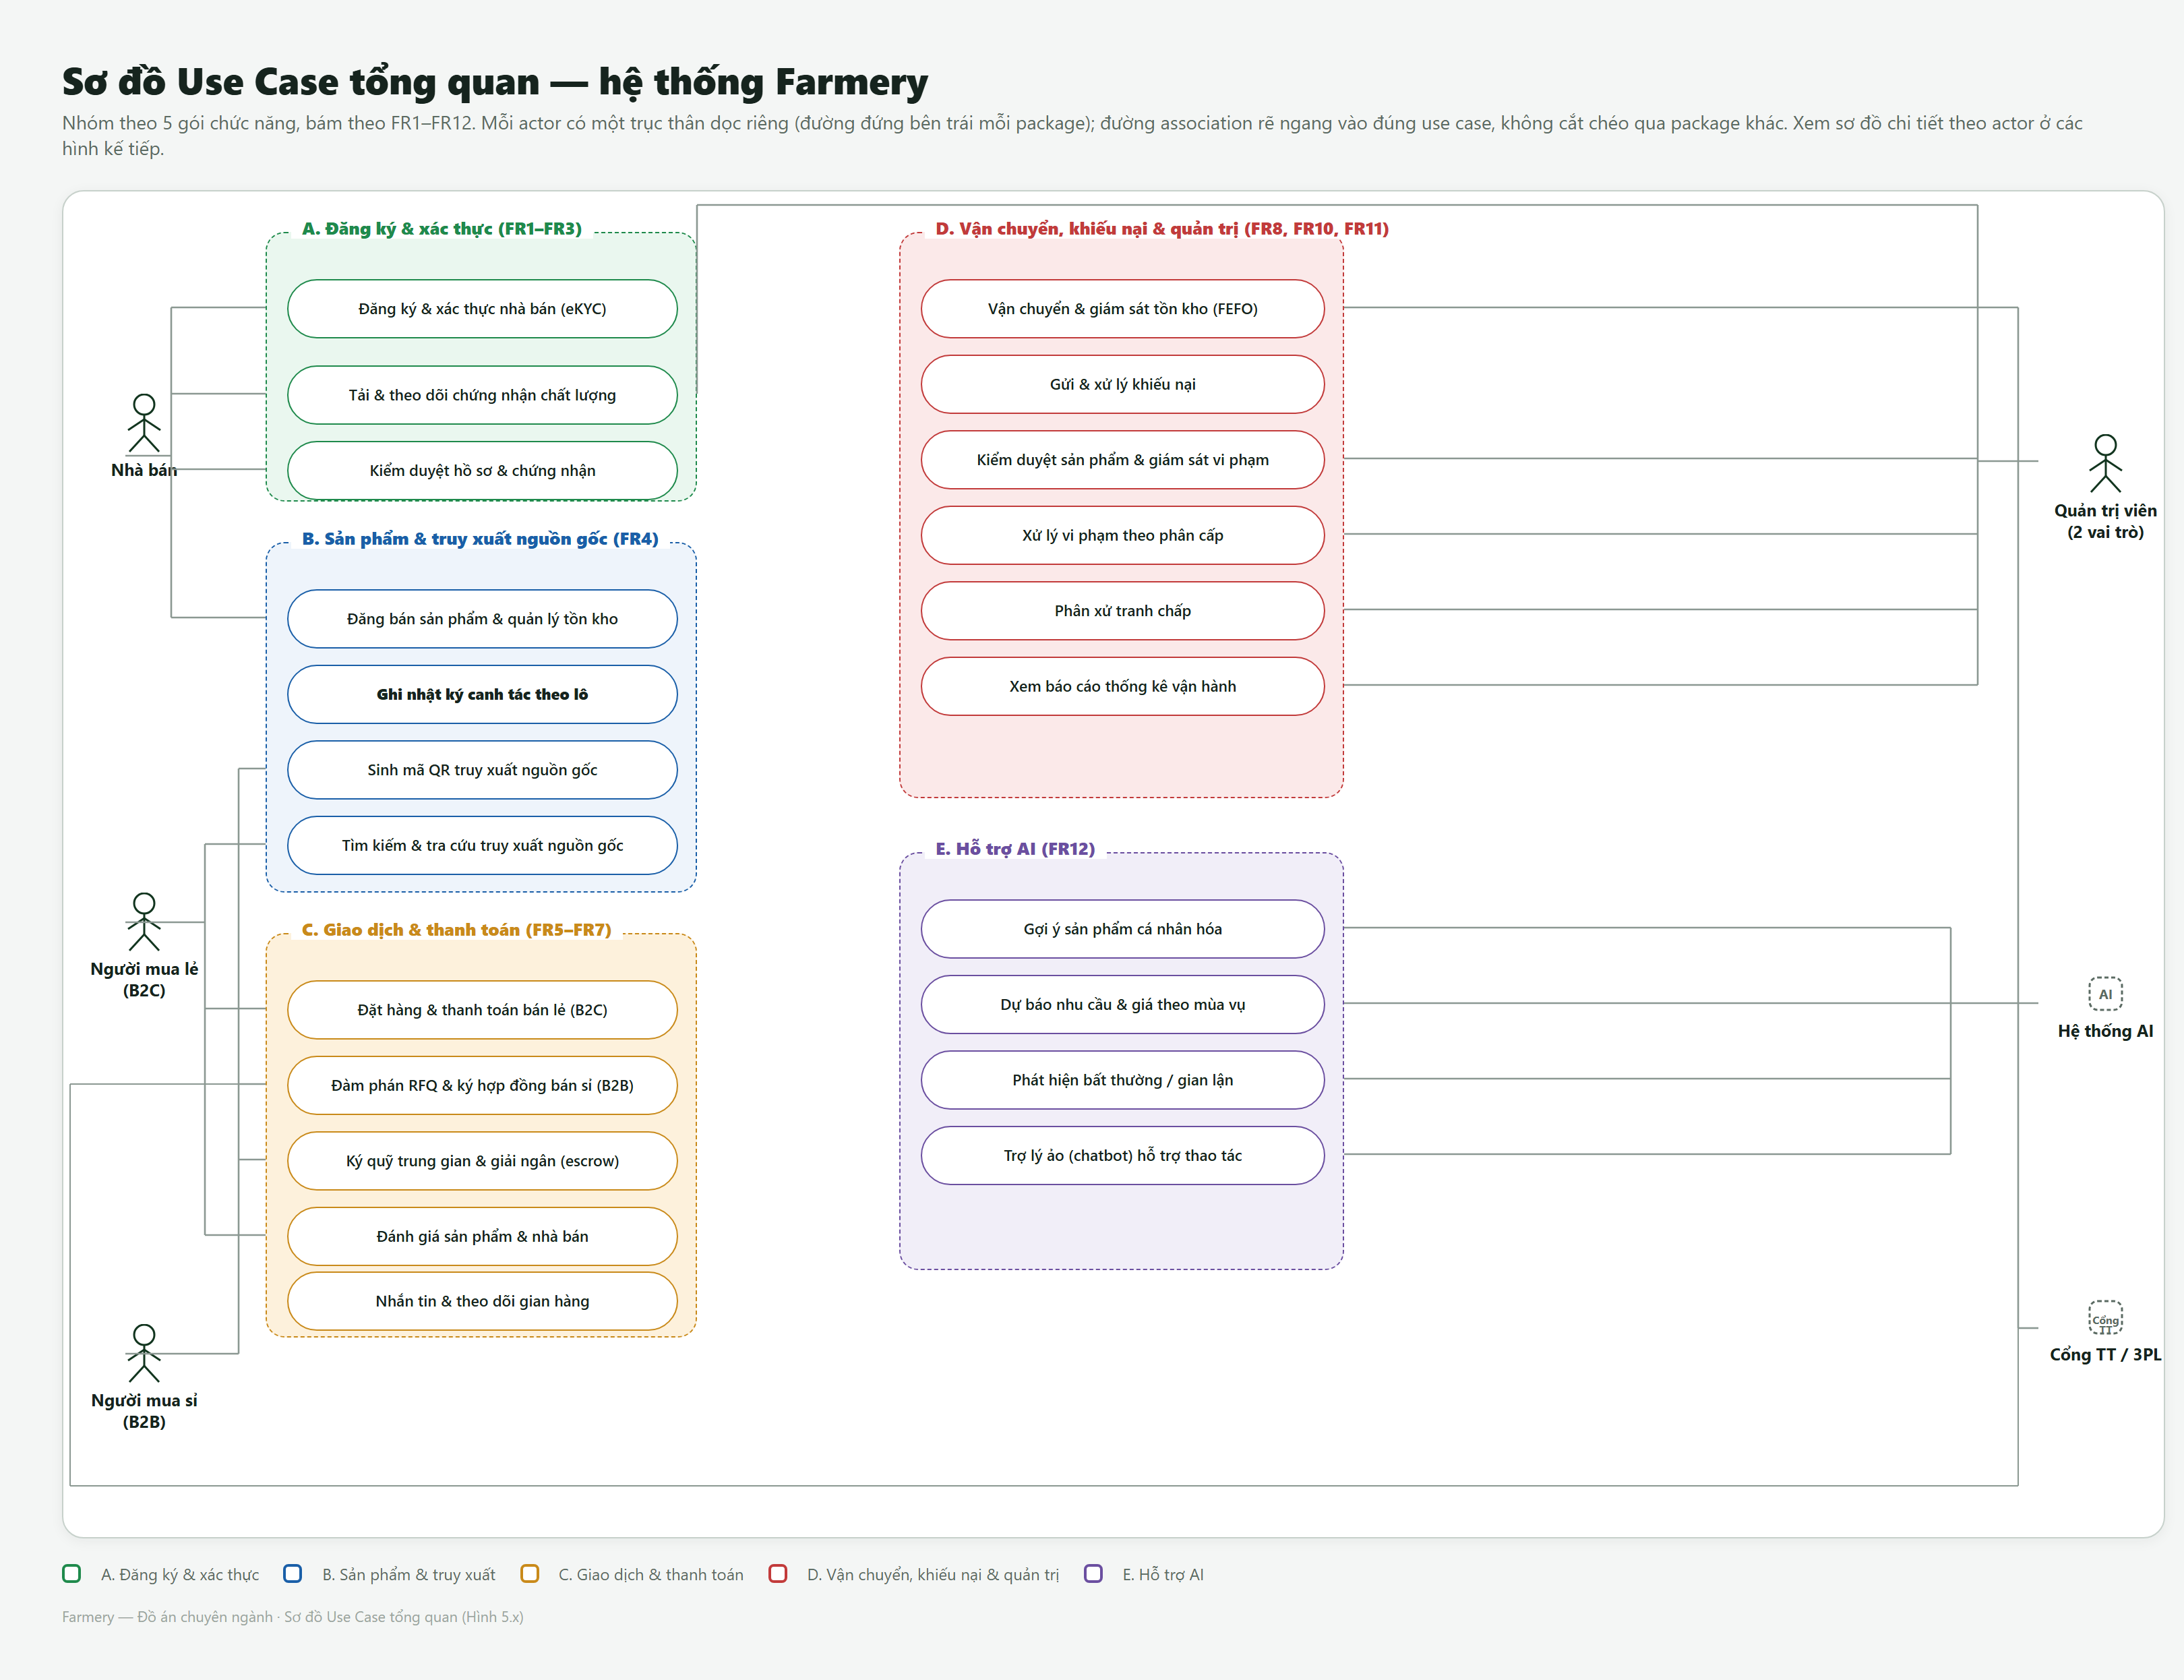
\includegraphics[width=\textwidth]{image/comparison/usecase-overview.png}
\caption{Sơ đồ Use Case tổng quan hệ thống Farmery}
\label{fig:usecase-overview}
\end{figure}

\subsubsection*{Sơ đồ use case chi tiết theo tác nhân}

Hình~\ref{fig:usecase-nhaban} minh họa chi tiết các use case của Nhà cung cấp quanh nhóm sản phẩm và truy xuất nguồn gốc (FR4), gồm đầy đủ quan hệ \texttt{<<include>>} (bắt buộc) và \texttt{<<extend>>} (mở rộng có điều kiện) theo chuẩn UML.

\begin{figure}[H]
\centering
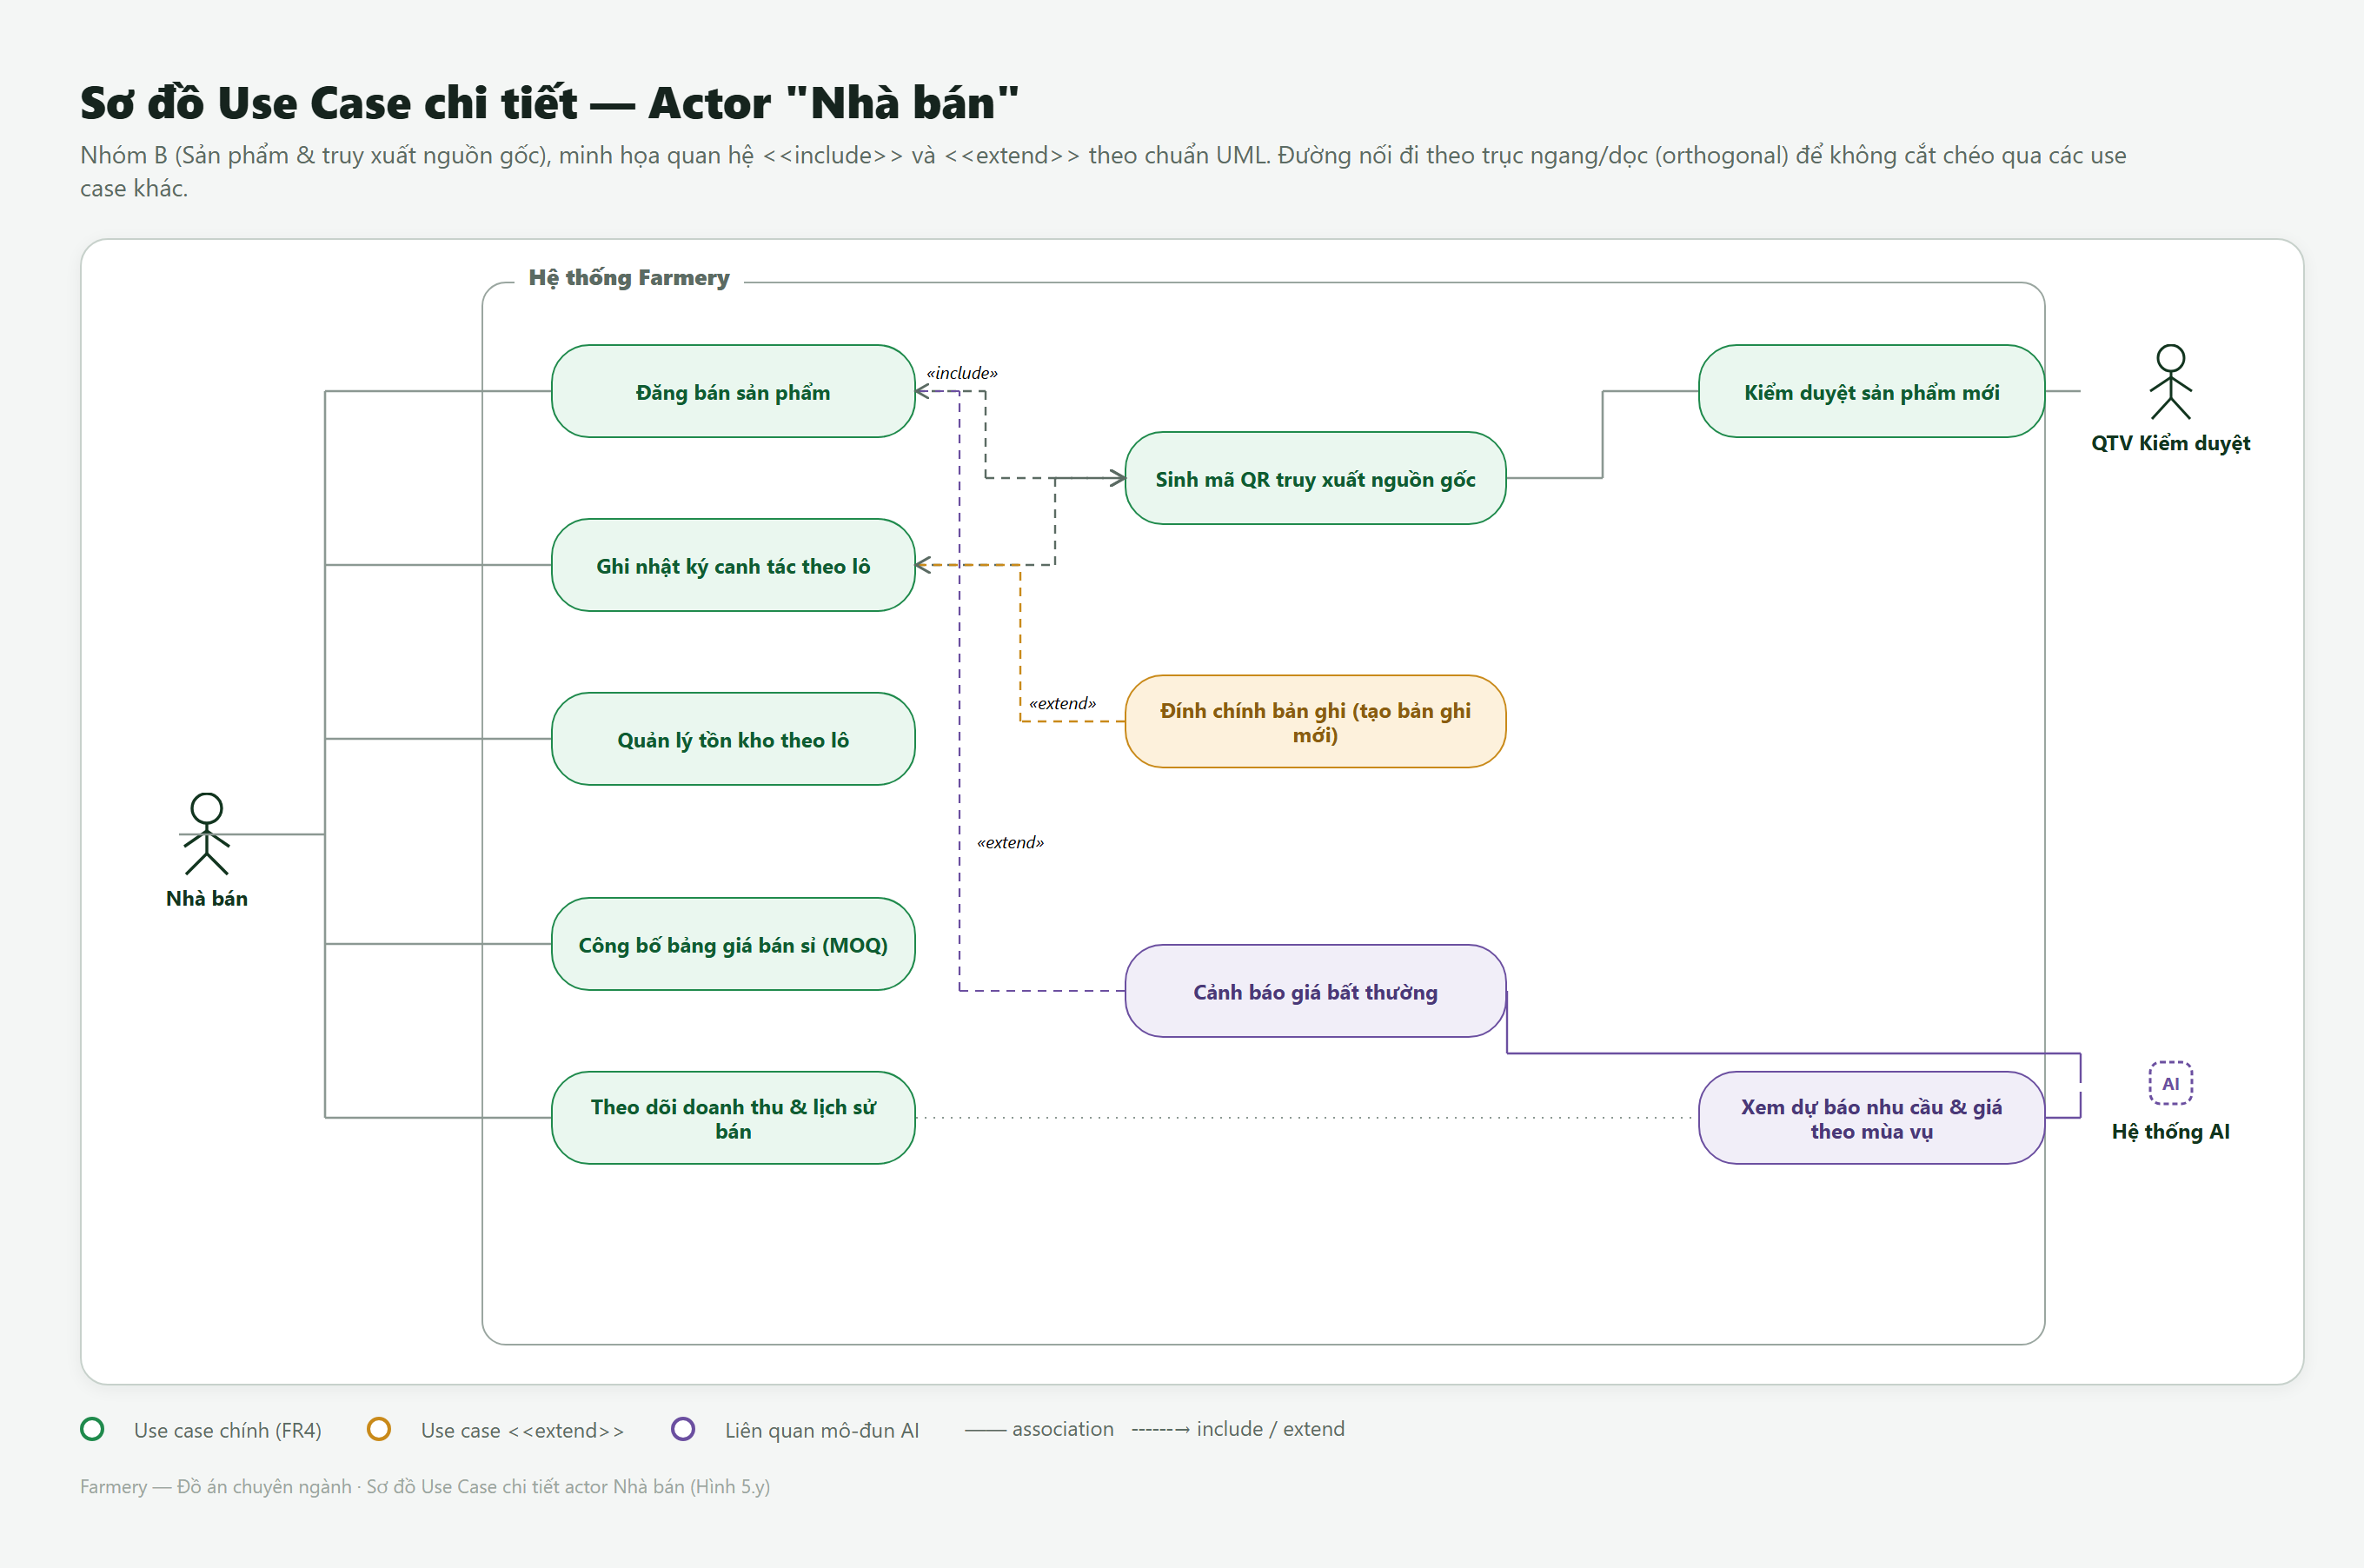
\includegraphics[width=\textwidth]{image/comparison/usecase-nha-ban.png}
\caption{Sơ đồ Use Case chi tiết --- tác nhân Nhà cung cấp}
\label{fig:usecase-nhaban}
\end{figure}

Hình~\ref{fig:usecase-khachle} minh họa hành trình mua hàng bán lẻ đầy đủ của Khách lẻ (FR5).

\begin{figure}[H]
\centering
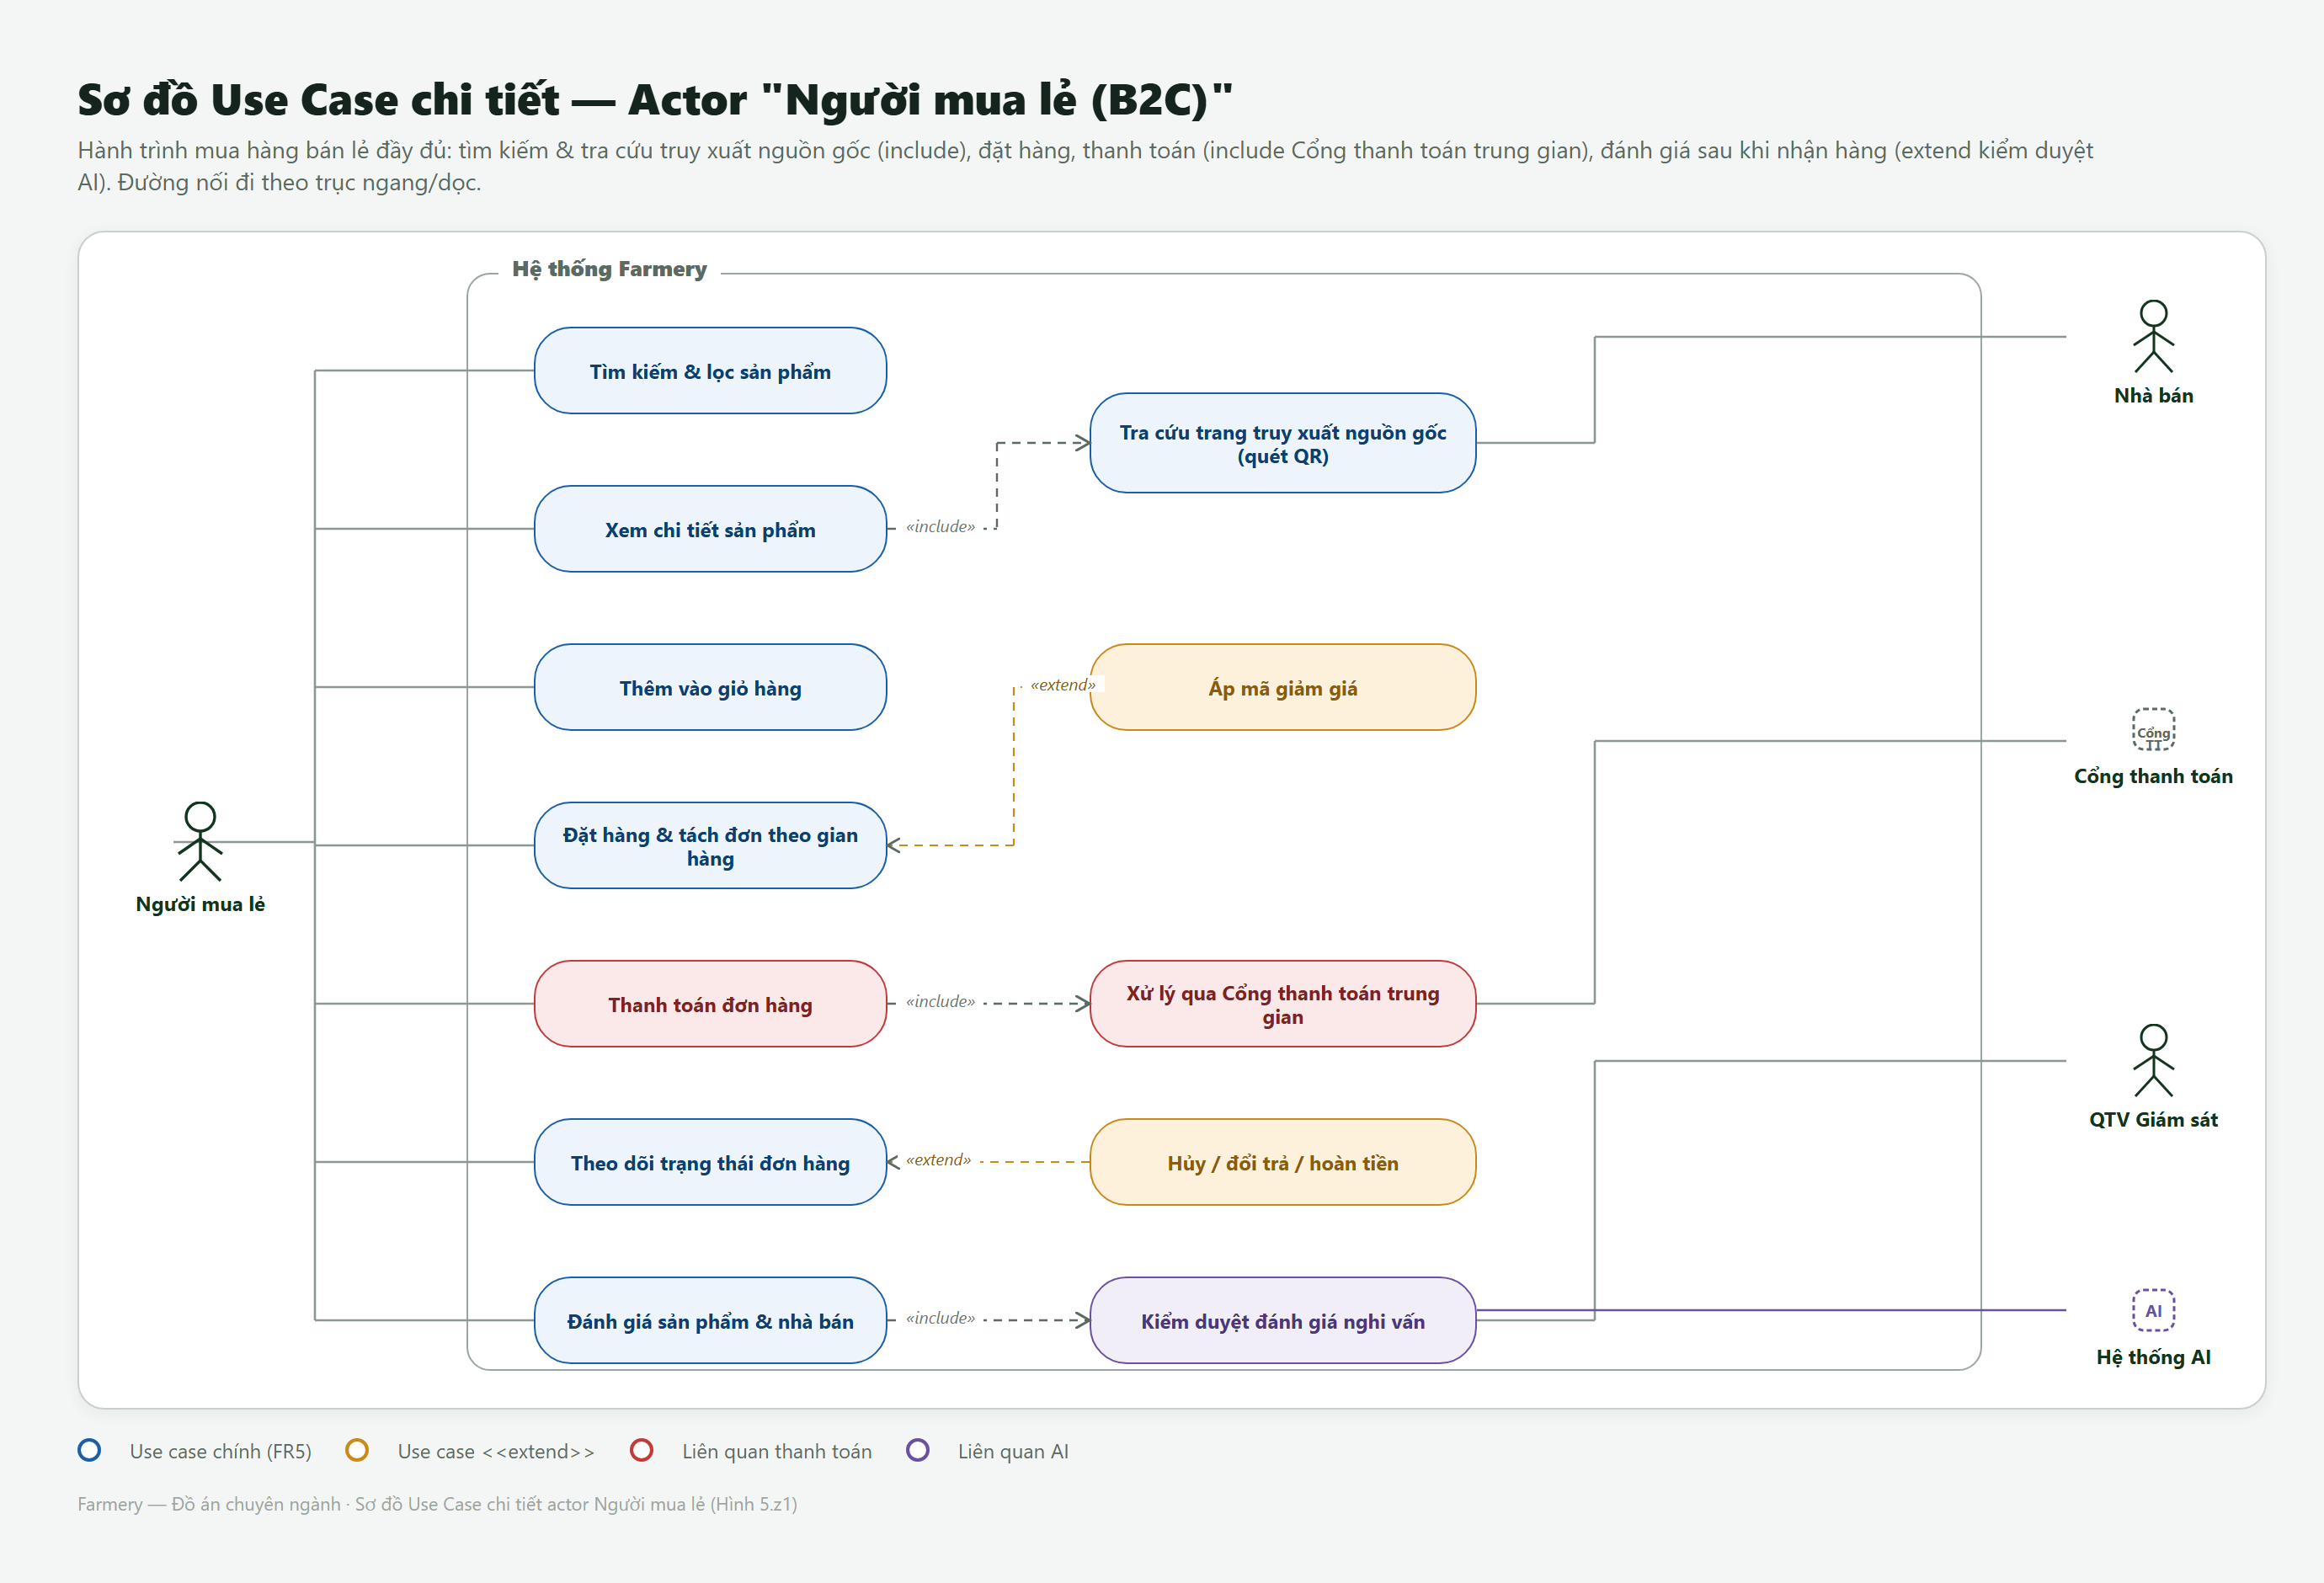
\includegraphics[width=\textwidth]{image/comparison/usecase-nguoi-mua-le.png}
\caption{Sơ đồ Use Case chi tiết --- tác nhân Khách lẻ}
\label{fig:usecase-khachle}
\end{figure}

Hình~\ref{fig:usecase-khachsi} minh họa luồng yêu cầu báo giá, hợp đồng điện tử, ký quỹ và giao hàng theo đợt của Khách sỉ (FR6, FR7).

\begin{figure}[H]
\centering
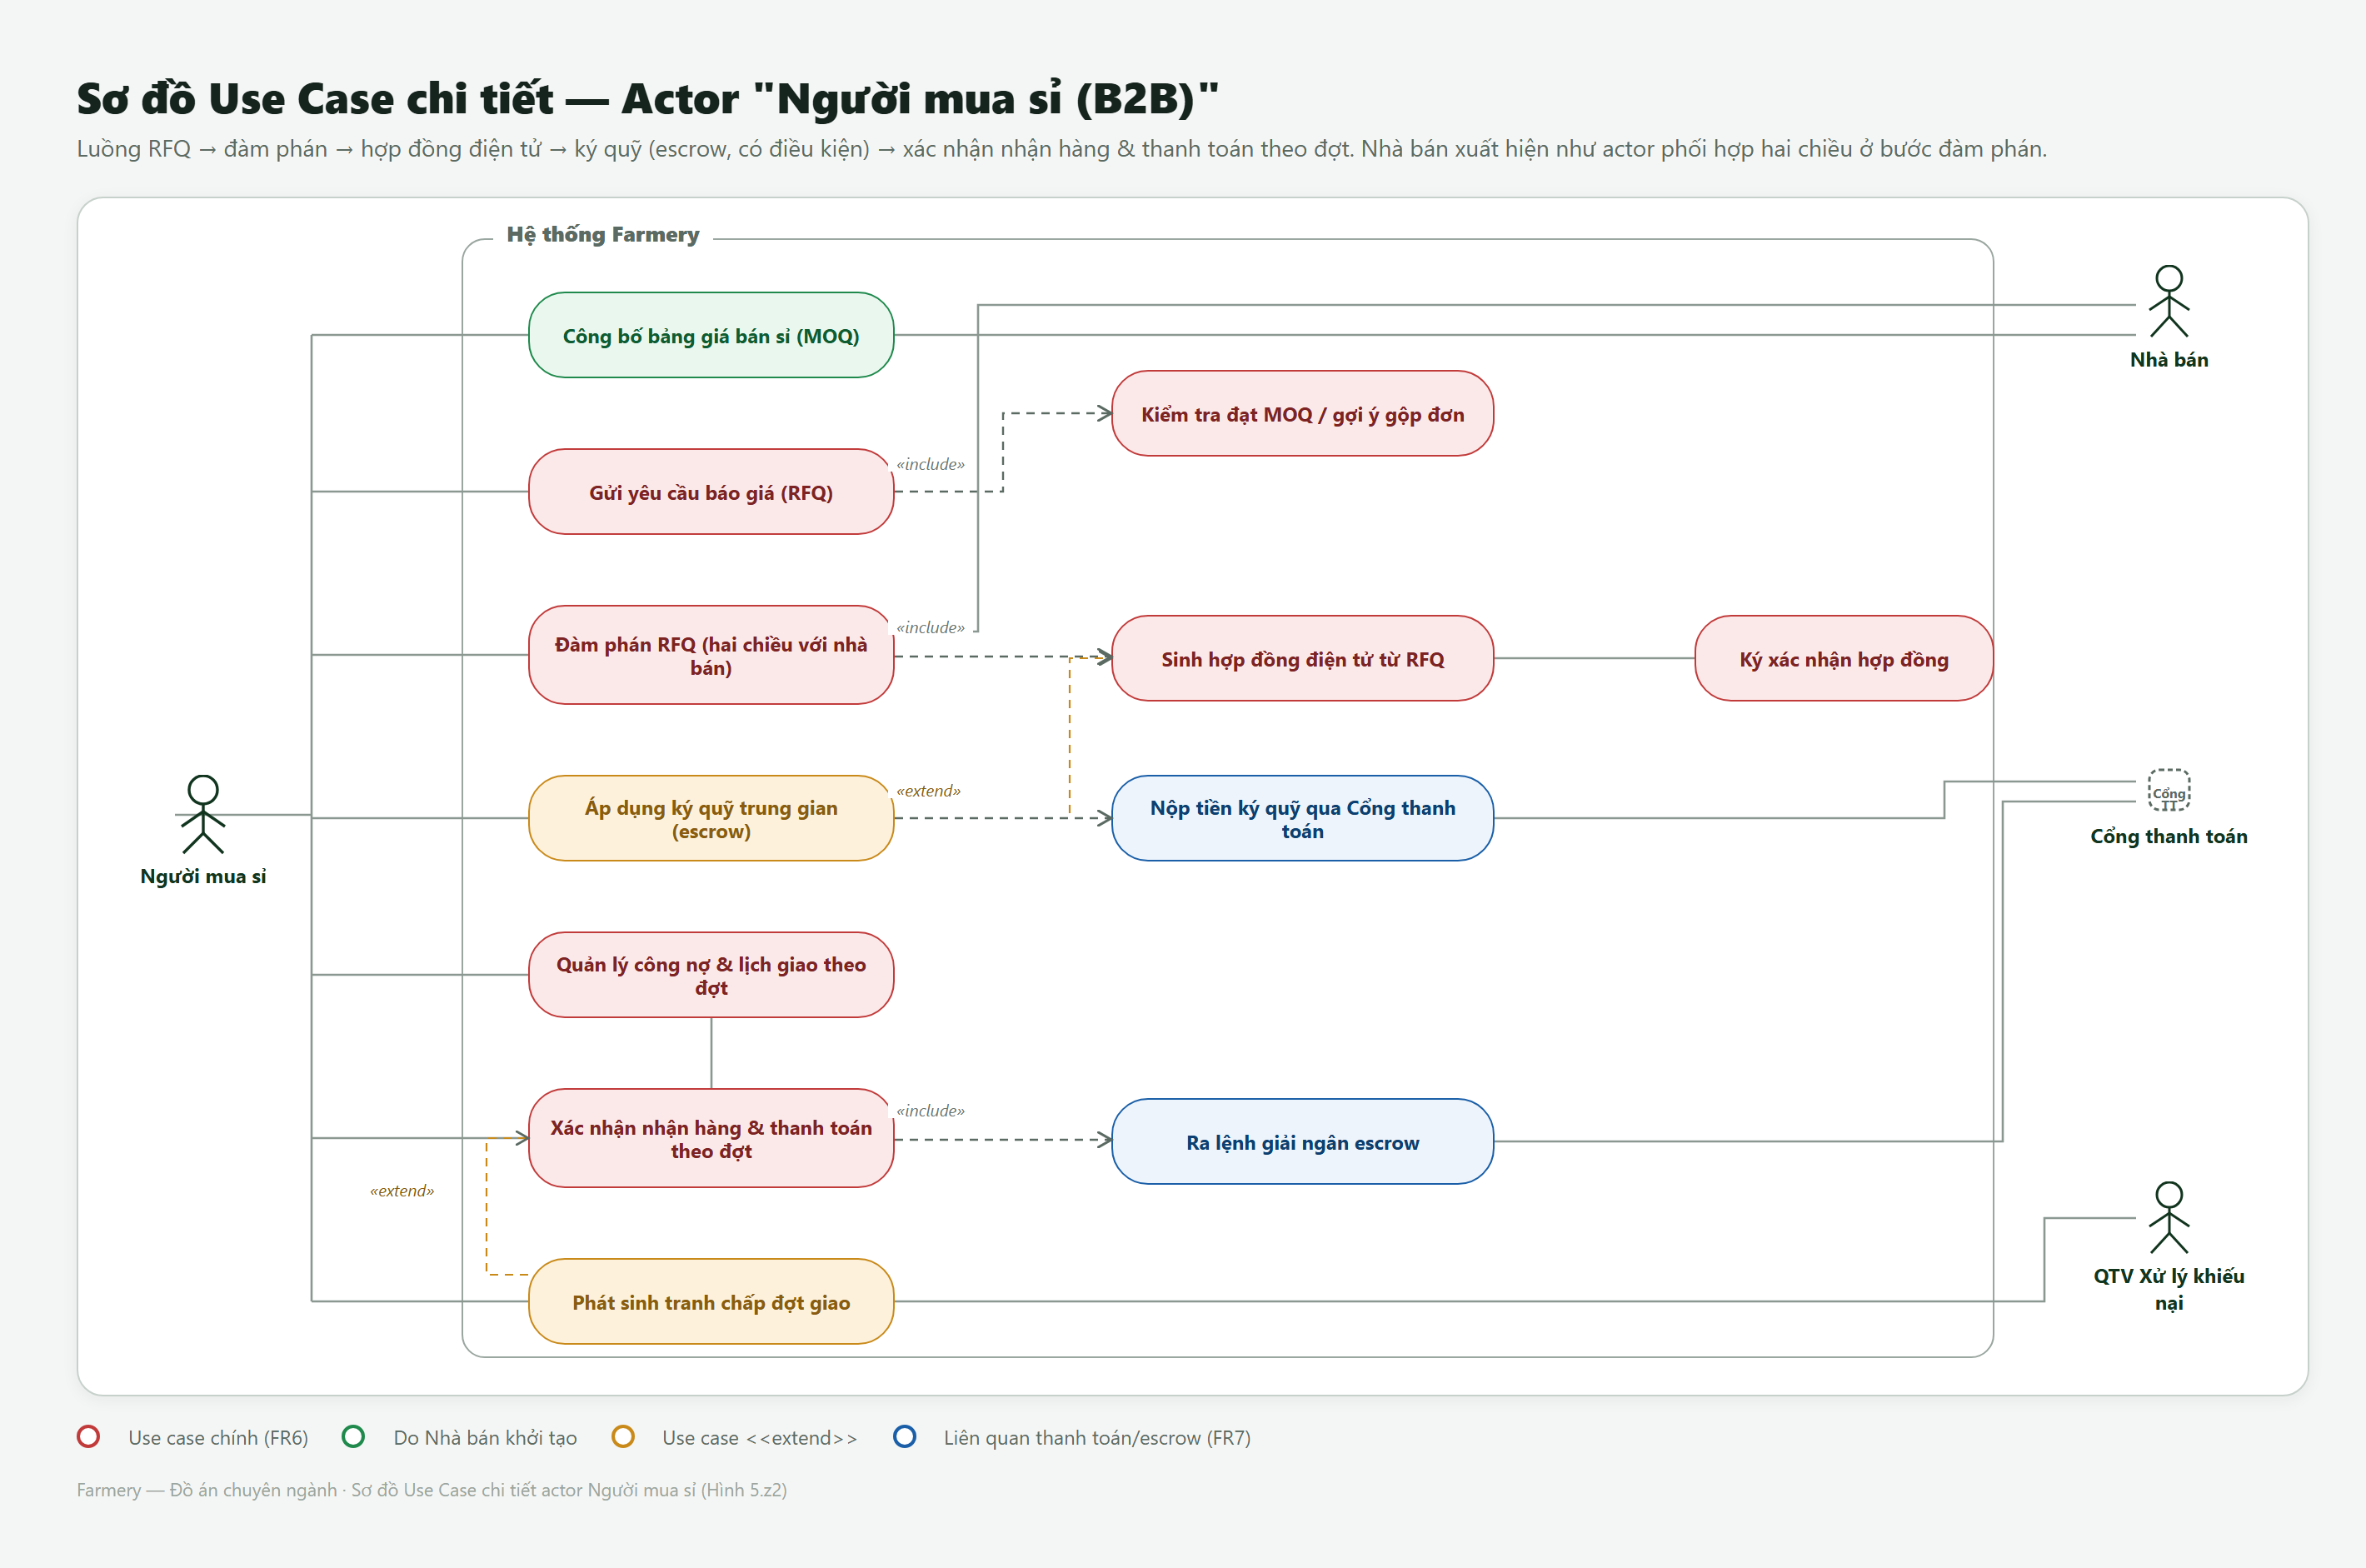
\includegraphics[width=\textwidth]{image/comparison/usecase-nguoi-mua-si.png}
\caption{Sơ đồ Use Case chi tiết --- tác nhân Khách sỉ}
\label{fig:usecase-khachsi}
\end{figure}

% CẢNH BÁO: hình dưới đây (usecase-quan-tri-vien.png) hiện vẽ theo giả định
% 5 vai trò admin con — CẦN VẼ LẠI cho khớp đúng 2 vai trò
% (admin_moderator, admin_ops) trước khi dùng chính thức. Xem mục "Việc cần
% xác nhận" ở cuối file.
\begin{figure}[H]
\centering
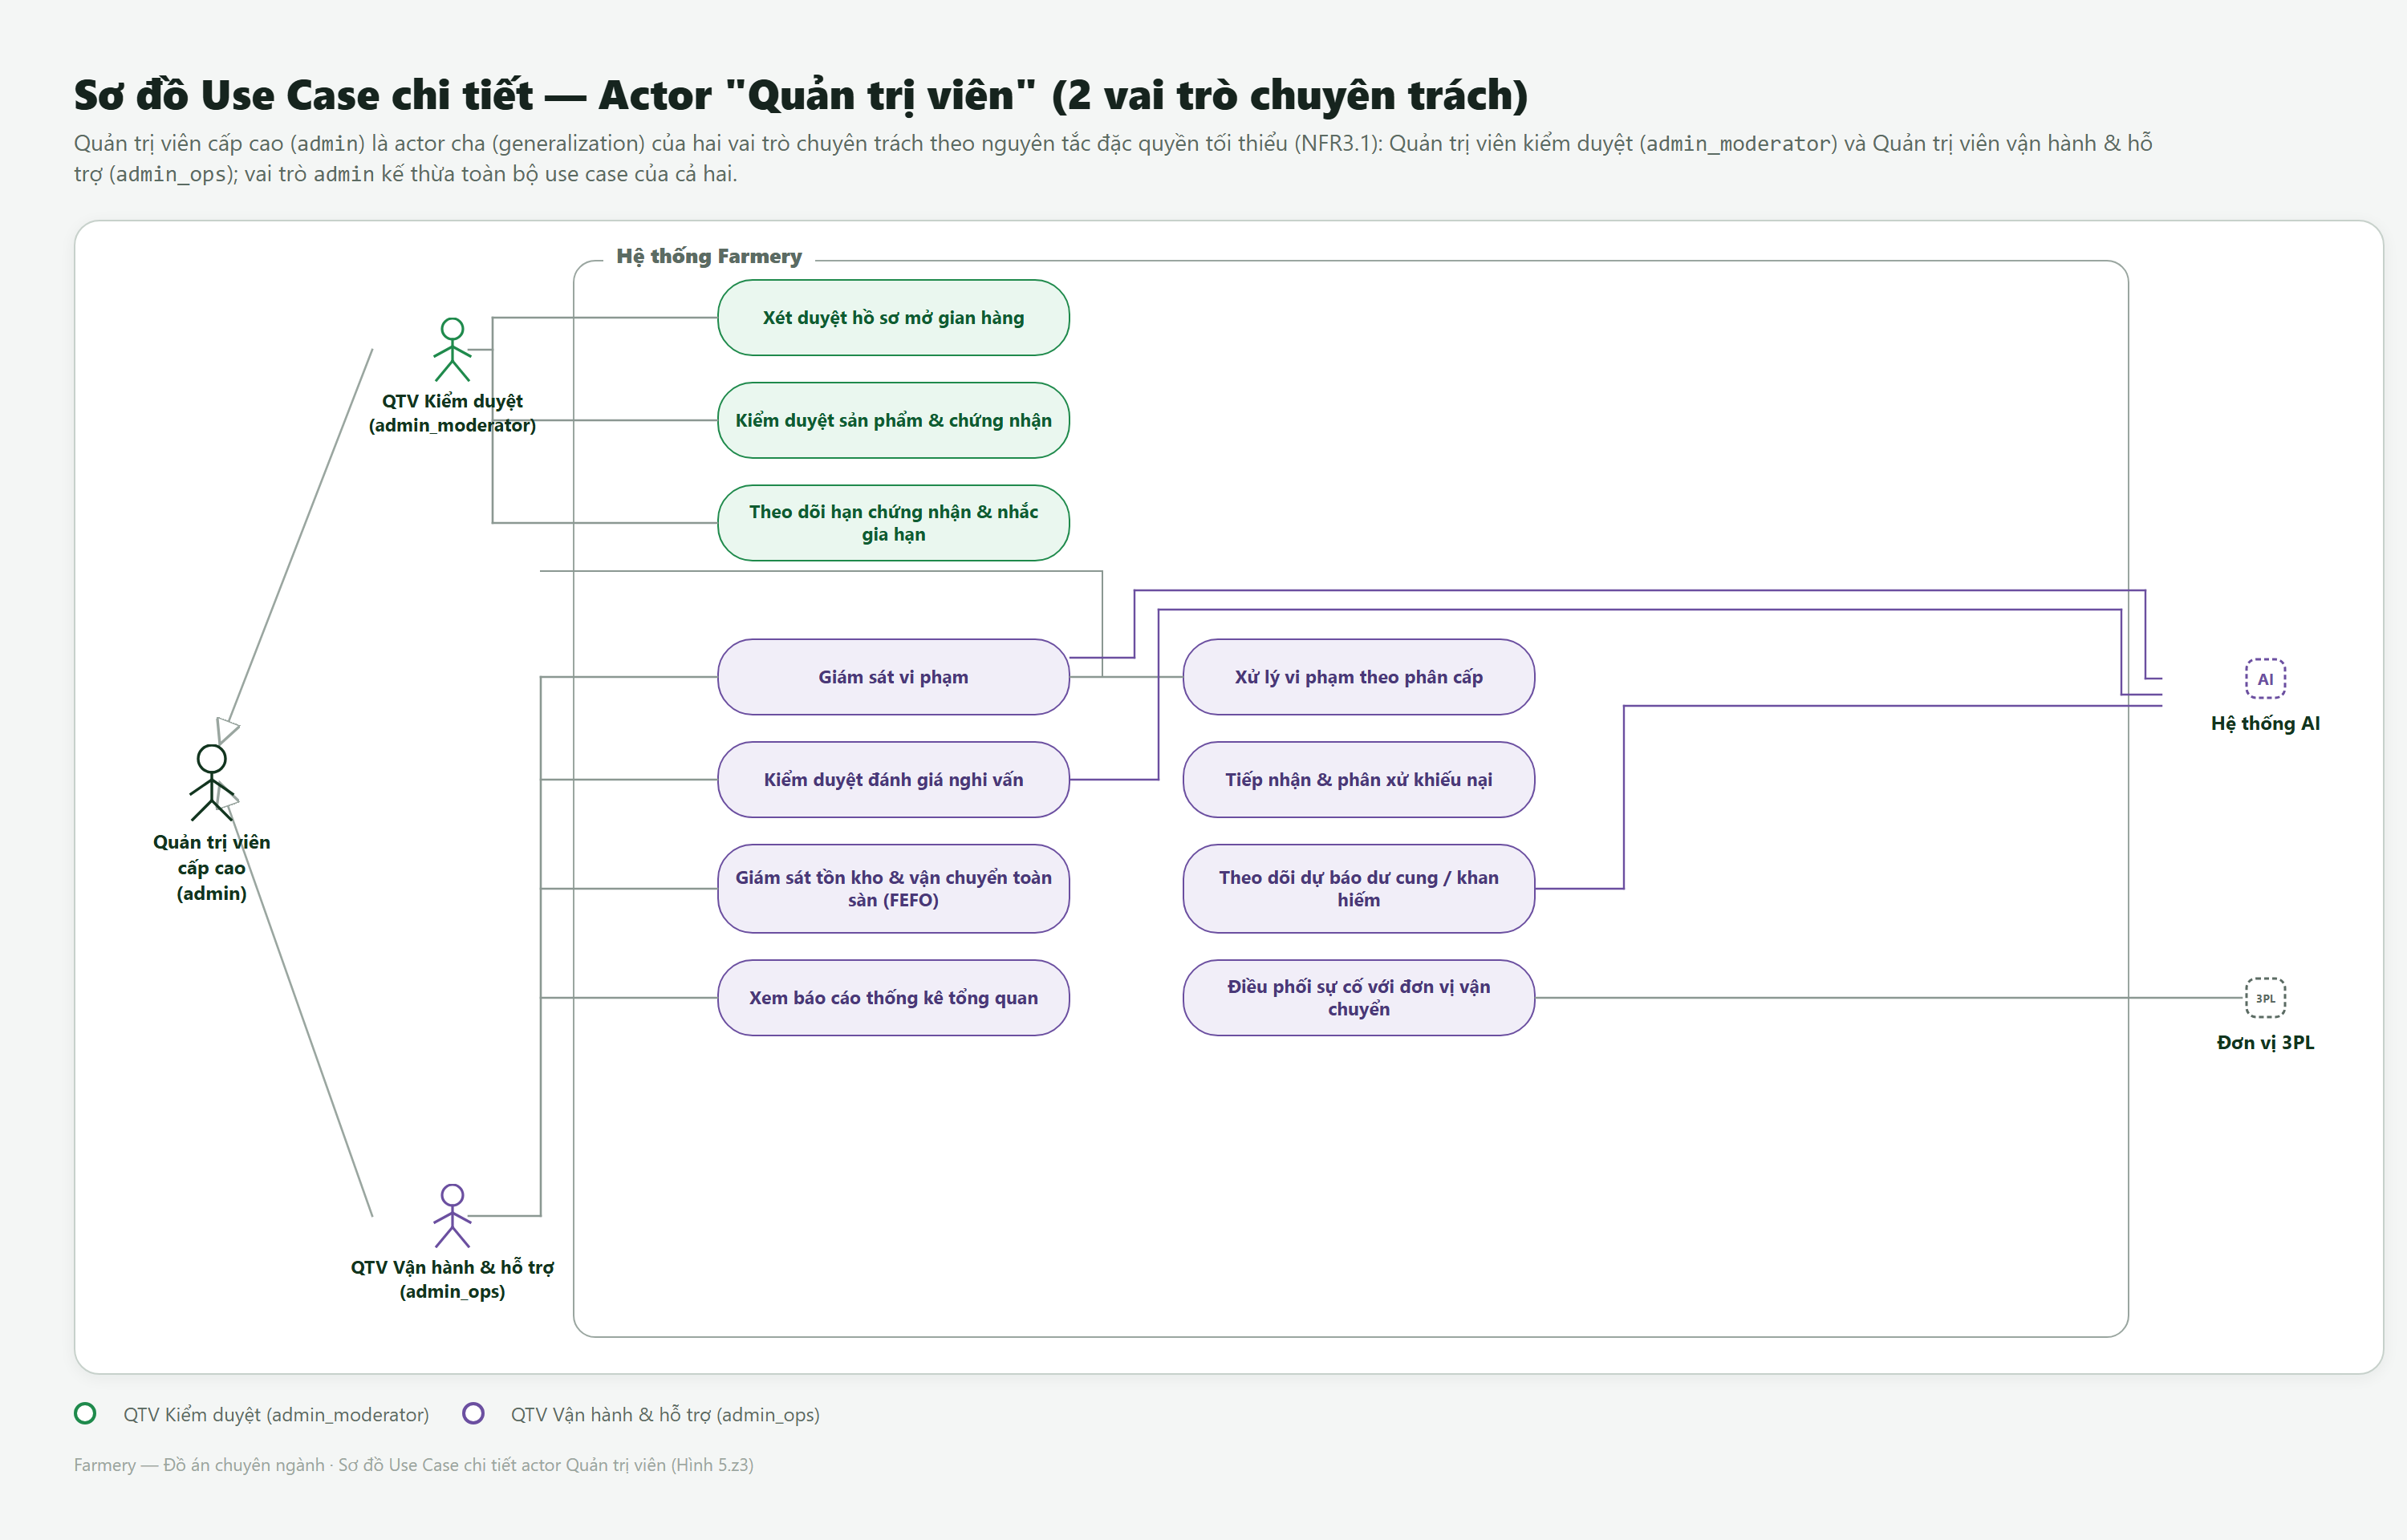
\includegraphics[width=\textwidth]{image/comparison/usecase-quan-tri-vien.png}
\caption{Sơ đồ Use Case chi tiết --- tác nhân Quản trị viên (bản nháp, cần vẽ lại theo đúng 2 vai trò admin\_moderator/admin\_ops)}
\label{fig:usecase-quantri}
\end{figure}

\subsubsection*{Bảng đặc tả các use case chính}

Các use case dưới đây được chọn đại diện cho mọi loại actor và loại luồng: thao tác đơn giản (UC-B2), luồng có sinh dữ liệu tự động (UC-B3), luồng có actor phụ bên ngoài (UC-C4, UC-D7), luồng nhiều bước có điều kiện rẽ nhánh (UC-D4), và luồng có AI hỗ trợ (UC-C7).

\begin{center}
\renewcommand{\arraystretch}{1.2}
\begin{longtable}{L{2.6cm} L{11.5cm}}
\caption{Đặc tả use case UC-B2 --- Ghi nhật ký canh tác theo lô}
\label{tab:uc-b2} \\
\toprule
\rowcolor{tblheadbg}
\multicolumn{2}{l}{\textbf{UC-B2: Ghi nhật ký canh tác theo lô}} \\
\midrule
\endfirsthead
\bottomrule
\endfoot
\textbf{Actor chính} & Nhà cung cấp (\texttt{seller}) \\
\rowcolor{tblaltbg}
\textbf{Tiền điều kiện} & Nhà cung cấp đã xác thực (trạng thái ``Đã xác thực''); đã tạo sản phẩm/lô hàng tương ứng (UC-B1) \\
\textbf{Luồng chính} &
1. Nhà cung cấp chọn lô hàng cần ghi nhật ký.\newline
2. Nhập giai đoạn canh tác (gieo trồng/chăm sóc/thu hoạch), ngày tháng, mô tả hoạt động.\newline
3. Tải ảnh minh chứng (nếu có).\newline
4. Hệ thống lưu bản ghi, gắn với lô tương ứng, đánh dấu thời điểm tạo (bất biến, không cho sửa trực tiếp --- NFR9.1).\newline
5. Nếu đủ điều kiện tối thiểu (≥1 bản ghi + ảnh sản phẩm thật), chuyển sản phẩm sang trạng thái đủ điều kiện xét duyệt công khai (UC-B4). \\
\rowcolor{tblaltbg}
\textbf{Luồng thay thế/ngoại lệ} &
4a. Cần đính chính bản ghi cũ: hệ thống không cho sửa trực tiếp, chỉ tạo bản ghi mới kèm ghi chú đính chính (NFR9.1). \\
\textbf{Hậu điều kiện} & Bản ghi được lưu vĩnh viễn (append-only), sẵn sàng hiển thị trên trang truy xuất công khai sau khi sản phẩm được duyệt. \\
\end{longtable}
\end{center}

\begin{center}
\renewcommand{\arraystretch}{1.2}
\begin{longtable}{L{2.6cm} L{11.5cm}}
\caption{Đặc tả use case UC-B3 --- Hệ thống sinh mã QR truy xuất nguồn gốc}
\label{tab:uc-b3} \\
\toprule
\rowcolor{tblheadbg}
\multicolumn{2}{l}{\textbf{UC-B3: Hệ thống sinh mã QR truy xuất nguồn gốc}} \\
\midrule
\endfirsthead
\bottomrule
\endfoot
\textbf{Actor chính} & Hệ thống (tự động, kích hoạt bởi UC-B4 khi quản trị viên kiểm duyệt duyệt sản phẩm) \\
\rowcolor{tblaltbg}
\textbf{Tiền điều kiện} & Sản phẩm/lô hàng đã qua kiểm duyệt và đạt điều kiện tối thiểu \\
\textbf{Luồng chính} &
1. Sinh mã định danh duy nhất theo nguyên lý GS1 (GTIN + batch/lot).\newline
2. Sinh mã QR liên kết tới trang truy xuất công khai.\newline
3. Trang truy xuất tổng hợp hồ sơ nhà cung cấp, chứng nhận đã duyệt, nhật ký canh tác, các mốc vận chuyển liên quan.\newline
4. Gắn mã QR vào trang sản phẩm, có thể in lên bao bì. \\
\rowcolor{tblaltbg}
\textbf{Luồng thay thế/ngoại lệ} & 1a. Lô đã có mã QR từ trước (do đính chính): không sinh mã mới, chỉ cập nhật nội dung trang truy xuất. \\
\textbf{Hậu điều kiện} & Mã QR khả dụng, quét được, dẫn tới trang truy xuất công khai đầy đủ và cập nhật. \\
\end{longtable}
\end{center}

\begin{center}
\renewcommand{\arraystretch}{1.2}
\begin{longtable}{L{2.6cm} L{11.5cm}}
\caption{Đặc tả use case UC-C4 --- Thanh toán đơn hàng bán lẻ}
\label{tab:uc-c4} \\
\toprule
\rowcolor{tblheadbg}
\multicolumn{2}{l}{\textbf{UC-C4: Thanh toán đơn hàng bán lẻ}} \\
\midrule
\endfirsthead
\bottomrule
\endfoot
\textbf{Actor chính} & Khách lẻ (\texttt{buyer\_retail}) \\
\rowcolor{tblaltbg}
\textbf{Actor phụ} & Cổng thanh toán trung gian \\
\textbf{Tiền điều kiện} & Đơn hàng đã được tạo, đang chờ thanh toán \\
\rowcolor{tblaltbg}
\textbf{Luồng chính} &
1. Chọn phương thức thanh toán (COD/chuyển khoản-VietQR/ví điện tử).\newline
2. Nếu trực tuyến: hệ thống chuyển yêu cầu tới cổng thanh toán trung gian.\newline
3. Cổng thanh toán xử lý, trả kết quả.\newline
4. Hệ thống xác nhận đơn, tạm trừ tồn kho.\newline
5. Thông báo cho bộ phận đóng gói chuẩn bị hàng. \\
\textbf{Luồng thay thế/ngoại lệ} &
3a. Thanh toán thất bại: đơn giữ trạng thái chờ tối đa 15 phút rồi tự hủy, giải phóng tồn kho.\newline
1a. Chọn COD: bỏ qua bước 2--3, xác nhận ngay.\newline
4a. Nhiều đơn vượt tồn kho còn lại: ưu tiên đơn xác nhận thanh toán trước. \\
\rowcolor{tblaltbg}
\textbf{Hậu điều kiện} & Đơn chuyển trạng thái đã xác nhận (hoặc hủy nếu thất bại), tồn kho cập nhật đúng kết quả giao dịch. \\
\end{longtable}
\end{center}

\begin{center}
\renewcommand{\arraystretch}{1.2}
\begin{longtable}{L{2.6cm} L{11.5cm}}
\caption{Đặc tả use case UC-D4 --- Sinh hợp đồng điện tử từ RFQ đã thống nhất}
\label{tab:uc-d4} \\
\toprule
\rowcolor{tblheadbg}
\multicolumn{2}{l}{\textbf{UC-D4: Sinh hợp đồng điện tử từ RFQ đã thống nhất}} \\
\midrule
\endfirsthead
\bottomrule
\endfoot
\textbf{Actor chính} & Hệ thống (tự động, sau khi Nhà cung cấp và Khách sỉ hoàn tất đàm phán) \\
\rowcolor{tblaltbg}
\textbf{Tiền điều kiện} & RFQ đã được nhà cung cấp xác nhận/điều chỉnh, hai bên thống nhất số lượng, đơn giá, lịch giao qua kênh nhắn tin nội bộ \\
\textbf{Luồng chính} &
1. Lấy thông tin đã thống nhất (sản phẩm, số lượng, đơn giá theo bậc, lịch giao, điều kiện thanh toán).\newline
2. Điền vào mẫu hợp đồng chuẩn, gồm điều khoản phạt vi phạm và thanh toán/công nợ.\newline
3. Gửi hợp đồng nháp cho cả hai bên xem trước khi ký (UC-D5). \\
\rowcolor{tblaltbg}
\textbf{Luồng thay thế/ngoại lệ} & 1a. Giá trị hợp đồng vượt ngưỡng quy định: đánh dấu thuộc diện áp dụng ký quỹ trung gian (FR7.3). \\
\textbf{Hậu điều kiện} & Hợp đồng điện tử ở trạng thái ``chờ ký'', lưu lịch sử phiên bản. \\
\end{longtable}
\end{center}

\begin{center}
\renewcommand{\arraystretch}{1.2}
\begin{longtable}{L{2.6cm} L{11.5cm}}
\caption{Đặc tả use case UC-D7 --- Xác nhận nhận hàng và thanh toán theo đợt}
\label{tab:uc-d7} \\
\toprule
\rowcolor{tblheadbg}
\multicolumn{2}{l}{\textbf{UC-D7: Xác nhận nhận hàng và thanh toán theo đợt}} \\
\midrule
\endfirsthead
\bottomrule
\endfoot
\textbf{Actor chính} & Khách sỉ (\texttt{buyer\_wholesale}) \\
\rowcolor{tblaltbg}
\textbf{Actor phụ} & Cổng thanh toán trung gian \\
\textbf{Tiền điều kiện} & Nhà cung cấp đã giao hàng đợt tương ứng theo hợp đồng đã ký; hệ thống đã sinh hóa đơn cho đợt giao đó \\
\rowcolor{tblaltbg}
\textbf{Luồng chính} &
1. Kiểm tra và xác nhận đã nhận đủ hàng đúng cam kết của đợt giao.\newline
2. Thanh toán theo kỳ hạn công nợ đã thỏa thuận.\newline
3. Nếu hợp đồng có ký quỹ: hệ thống ra lệnh cho cổng thanh toán giải ngân cho nhà cung cấp ngay tại bước xác nhận này.\newline
4. Nhà cung cấp theo dõi doanh thu/lịch sử bán sỉ cập nhật. \\
\textbf{Luồng thay thế/ngoại lệ} &
1a. Không giao đủ số lượng/đúng lịch: áp dụng điều khoản phạt, ghi vào lịch sử uy tín.\newline
2a. Chậm thanh toán quá hạn: nhắc tự động, có thể tạm khóa quyền đặt RFQ mới.\newline
3a. Phát sinh tranh chấp về đợt giao đã ký quỹ: khoản ký quỹ giữ nguyên tại cổng thanh toán cho đến khi khiếu nại xử lý xong. \\
\rowcolor{tblaltbg}
\textbf{Hậu điều kiện} & Đợt giao chuyển trạng thái hoàn tất, công nợ cập nhật, tiền giải ngân cho nhà cung cấp (nếu có ký quỹ). \\
\end{longtable}
\end{center}

\begin{center}
\renewcommand{\arraystretch}{1.2}
\begin{longtable}{L{2.6cm} L{11.5cm}}
\caption{Đặc tả use case UC-C7 --- Kiểm duyệt đánh giá nghi vấn}
\label{tab:uc-c7} \\
\toprule
\rowcolor{tblheadbg}
\multicolumn{2}{l}{\textbf{UC-C7: Kiểm duyệt đánh giá nghi vấn}} \\
\midrule
\endfirsthead
\bottomrule
\endfoot
\textbf{Actor chính} & Quản trị viên vận hành (\texttt{admin\_ops}) \\
\rowcolor{tblaltbg}
\textbf{Actor phụ} & Hệ thống (luật ngưỡng giám sát bất thường, Chương~\ref{chap:coso}) \\
\textbf{Tiền điều kiện} & Người mua đã gửi đánh giá sau khi xác nhận nhận hàng \\
\rowcolor{tblaltbg}
\textbf{Luồng chính} &
1. Kiểm duyệt tự động sơ bộ (từ khóa cấm, liên kết đáng ngờ).\newline
2. Áp dụng luật ngưỡng để tìm dấu hiệu giả mạo/spam/thao túng uy tín.\newline
3. Không nghi ngờ: công khai ngay.\newline
4. Bị nghi ngờ: chuyển quản trị viên xem xét thủ công.\newline
5. Quyết định công khai hoặc ẩn.\newline
6. Cập nhật điểm uy tín tổng hợp (không tính đánh giá bị ẩn). \\
\textbf{Luồng thay thế/ngoại lệ} &
5a. Xác nhận đánh giá giả/vi phạm: ẩn, thông báo lý do, không tính điểm uy tín.\newline
5b. Phát hiện nhà cung cấp thao túng đánh giá: chuyển quy trình xử lý vi phạm (mục~\ref{sec:quytrinhnghiepvu}, Quản trị hệ thống). \\
\rowcolor{tblaltbg}
\textbf{Hậu điều kiện} & Đánh giá ở trạng thái công khai hoặc ẩn dứt điểm; điểm uy tín cập nhật chính xác. \\
\end{longtable}
\end{center}

% ============================================================
% VIỆC CẦN NHÓM XÁC NHẬN TRƯỚC KHI MERGE (QUAN TRỌNG):
%
% 1. *** VẼ LẠI DIAGRAM QUẢN TRỊ VIÊN ***: file tools/design/usecase-quan-
%    tri-vien.html hiện vẽ 5 vai trò admin con (moderator, compliance,
%    support, ops, inventory) — SAI so với RBAC thật chỉ có 2 vai trò
%    (admin_moderator, admin_ops) cộng admin super-admin. Cần sửa lại file
%    HTML này (gộp use case của 5 nhóm cũ thành 2 nhóm: admin_moderator
%    nhận nhóm kiểm duyệt; admin_ops nhận các nhóm còn lại: giám sát vi
%    phạm, khiếu nại, báo cáo, tồn kho/vận chuyển) trước khi render chính
%    thức bằng npm run shot.
% 2. Kiểm tra lại 4 file diagram còn lại (overview, nha-ban, nguoi-mua-le,
%    nguoi-mua-si) xem có tham chiếu nhầm actor admin nào theo giả định 5
%    vai trò cũ không — nếu overview.html có nhắc "Quản trị viên (5 vai
%    trò)" thì cần sửa thành "(2 vai trò)".
% 3. Đã đặc tả chi tiết 6/hơn 45 use case liệt kê — nếu giảng viên yêu cầu
%    đặc tả 100%, cần làm thêm theo đúng mẫu bảng này.
% 4. Xác nhận vị trí chèn đúng dòng "% TODO: vẽ use case diagram..." trong
%    chuong5-phantich-thietke.tex, mục sec:sddchitiet.
% 5. Cả 5 ảnh PNG (image/comparison/usecase-*.png) hiện CHƯA được render —
%    cần chạy `npm run shot` (hoặc lệnh render tương ứng) trong repo trước
%    khi biên dịch main.tex, nếu không \includegraphics sẽ báo lỗi thiếu
%    file.
% ============================================================
